\chapter{Results}
\label{results}
%[inline]{tons of pictures. easy pictures, hard pictures, why they're hard}
%DONE{methodology section, like how neural networks were used, opencv section in methodology. cpu and clock speed and rate of processing}

\section{Methodology}

%Opencv/environment/language
\subsection{Environment}
This project was done entirely in OpenCV 3.0 using their C++ libraries. The computer used for this project was running Windows 8.1 on a Intel i5-2500K CPU with a maximum clock speed of 4.1 GHz. The OpenCV libraries are widely used and support a large amount of languages and platforms, including Apple iOS, Android, OpenCL, CUDA, as well as Mac, Linux and PC, which means that the code is easily ported to most any platform \cite{OpenCVPlatforms}. The input images were all read from saved video files on disk, and fed one by one into this project's algorithm. 

%what data was used, where it came from, what was trained, etc.
\subsection{Dataset}
%JeneePlz
The data used for the results were a selection of videos from multiple white crosswalks and streets without crosswalks taken at and around street intersections. The videos were taken at multiple times of day ranging from early morning to early night. For each crosswalk, five videos were taken going the same direction across the crosswalk. The videos were a high angle, a low angle, walking on the left side, on the right side, and a walking in the center.  Videos were given categories: time of day, angle of video, type of crosswalk, color, crosswalk title, etc. Crosswalks were marked to be used only for training the neural network, and other crosswalks marked only to be used for evaluating results. The training set contained three hybrid crosswalks, six zebra crosswalks, and ten videos that did not include crosswalks. The result testing set contained three hybrid crosswalks, nine zebra crosswalks, and eighteen videos that did not include crosswalks. All data in the results section is generated from videos that were never used in the training process of the neural network. Over 14,000 stripelets were marked by hand as part of a crosswalk or not part of a crosswalk for use when training the neural network, and over 18,000 manually marked stripelets were used for the output. Each crosswalk video only used 20 frames, whereas videos without crosswalk may have used more. Hybrid crosswalks were included as well because they were working with the algorithm as well. 


%How Neural Networks are used here (explain some of the experimentation around different layers, and how they didn't do much)
\section{Neural Network Configuration}
%Jeneeplz
For this project, neural networks are used for the prediction of stripelets as either being part of a crosswalk or not. Neural networks require a set number of hidden layers with a set number of neurons, so some experimentation was done to determine these numbers. As shown in figure \ref{fig:Neural1png}, for this project, the final result was one hidden layer of 14 neurons. A supervised feedforward network trained using backpropagation was used for this project. This neural network configuration is one of the simpler configurations, and remains very effective. An unsupervised neural network configuration would not be as optimal for this same exact data because the outputs are known, allowing a supervised method to train more efficiently. A larger training set would likely be required for an unsupervised network. 

%D:\Users\SandyBridge\Dropbox\Thesis\My Paper Stuff\Results\Results of NN Training with diff neurons.xlsx
%    \begin{table}[t]
%%        \begin{longtable}{| r | r | r | r |}
 %       \hline
 %       Neurons in Hidden Layer & True Positive Rate & False Positive Rate & q-value \bigstrut\\
 %       \hline
 %       15 & 74.42\% & 2.36\% & 0.086 \bigstrut\\
 %       \hline
 %       \caption[Selected Neural Network Configuration Results]{Stripelet identification results from neural network training with selected hidden layer configuration}
 %       \label{tab:NN-HiddenLayersResults} 
 %       \end{longtable}
 %   \end{table}
 
 %TODO

There is no real consensus on exactly how many hidden layers and neurons should be used in the perfect neural network configuration. The different rules of thumb have been that no more than one hidden layer is typically needed, and the number of neurons should be between the number of inputs and the number of outputs, and layers must have more than one neuron\cite{Heaton:2008:INN:1502373}. With those being the guidelines, one hidden layer with a number of neurons mostly ranging from the number of inputs to the number of outputs was chosen with a range from 2 to 22 neurons in the hidden layer. Subsets of these training parameters were tried as well, with none having better results than using all eleven parameters. 

The neural network training of the crosswalk stripelets used many different input parameters to predict the output. The metric used for evaluating the parameters was finding the true positive and false negative rates, as well as the false discovery rate (also known as q-value). The true positive rate is calculated by dividing the number of crosswalk stripelets that were predicted correctly as stripelets over the total number of crosswalk stripelets. The false positive rate is calculated by dividing the number of non-crosswalk stripelets predicted as stripelets out of the total number of non-crosswalk stripelets. The q-value is found by dividing the number of false positives by the number of stripelets that were predicted to be part of a crosswalk. Table \ref{tab:nnresultsoverall} shows the neural network prediction rates over the entire result set. Only 16.6\% of the positively predicted stripelets were incorrect. 


As shown in appendix table \ref{tab:NN-HiddenLayersResultsAPP}, some configurations were better than others, but none by much. The configuration with the 14 neuron hidden layer had the lowest false positive rate of 3.12\%, so it was chosen as the configuration to be used for the rest of this project. This fits with the original assumption that the number of neurons should be between the number of inputs and outputs as shown in figure \ref{fig:Neural1png}. 

\begin{figure}[t]
\begin{center}
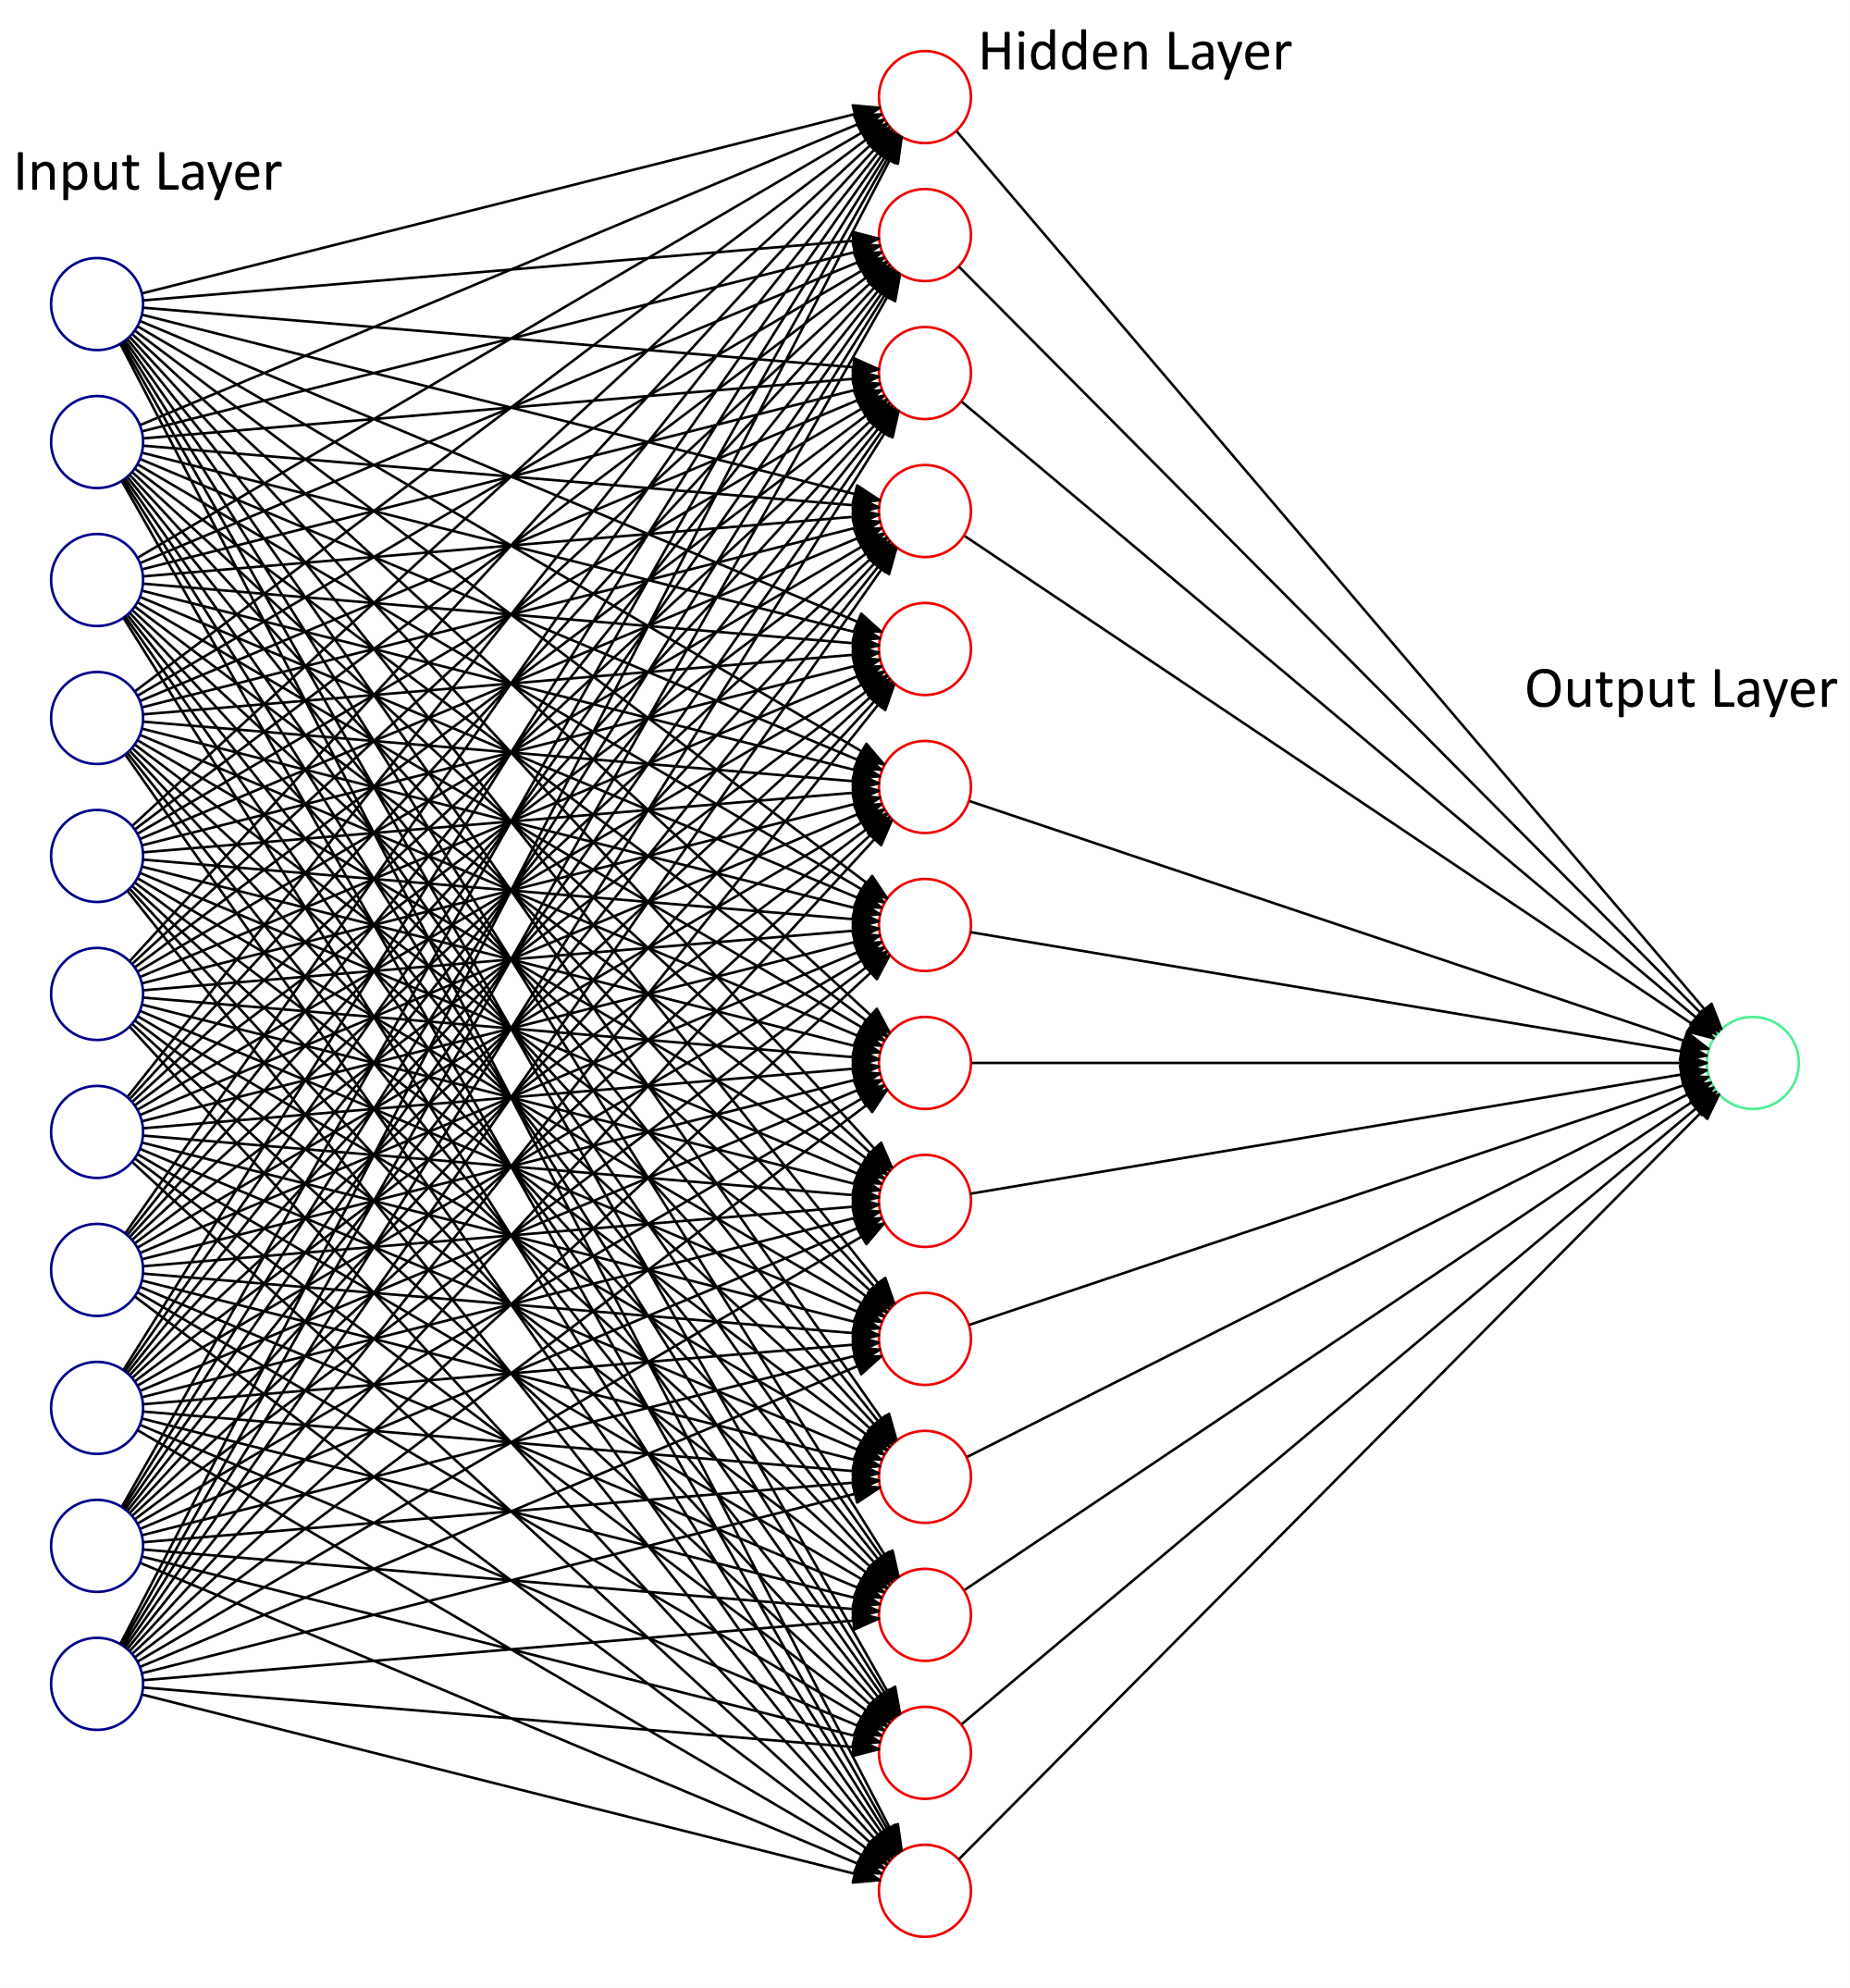
\includegraphics[width=10cm]{figures/ChosenNN3Small.png}
\captionfonts
\caption{Final neural network configuration showing input layers, hidden layers, and output layers}
\label{fig:Neural1png}
\end{center}
\end{figure}

    \begin{table}[t]
        \begin{longtable}{|r|r|r|r|}
        \caption{Neural Network results over stripelets in final dataset}
        \label{tab:nnresultsoverall}\\
        \hline
        Number of Stripelets & True Pos Rate & False Pos Rate & Q-Val \bigstrut\\
        \hline
        19461 & 77.61\% & 3.57\% & 0.1663 \bigstrut\\
        \hline
        \end{longtable}
    \end{table}

\clearpage





\section{Crosswalk Detection}
Once the neural network has finished culling stripelets, the remaining stripelets are then fed through the crosswalk detection algorithm. The results are again categorized by type of crosswalk, time of day, etc. 

\clearpage

\subsection{Effect of Different Video Angles}

There were five different angles used for the videos of the crosswalks, with 340 frames of video at each angle across many crosswalks. Examples of each angle are shown in figure \ref{fig:AllFiveAngles}. The low angle had worse correct prediction rates than the others, as shown in table \ref{tab:downbad}. The reason for this is that the cell phone camera was angled too low to capture enough stripelets for a positive identification. A few examples are given in figure \ref{fig:downBadPic}. The poor results from the bad video angle show that in an actual use case, that angle must be disallowed. The user could be trained to hold the cell phone camera at the proper angle, and if they did not, the sensors would allow the application to notify the user to adjust the camera angle. Because of this, the videos taken at that downward angle will be removed from the overall dataset. 

\begin{figure}[t]
\begin{center}
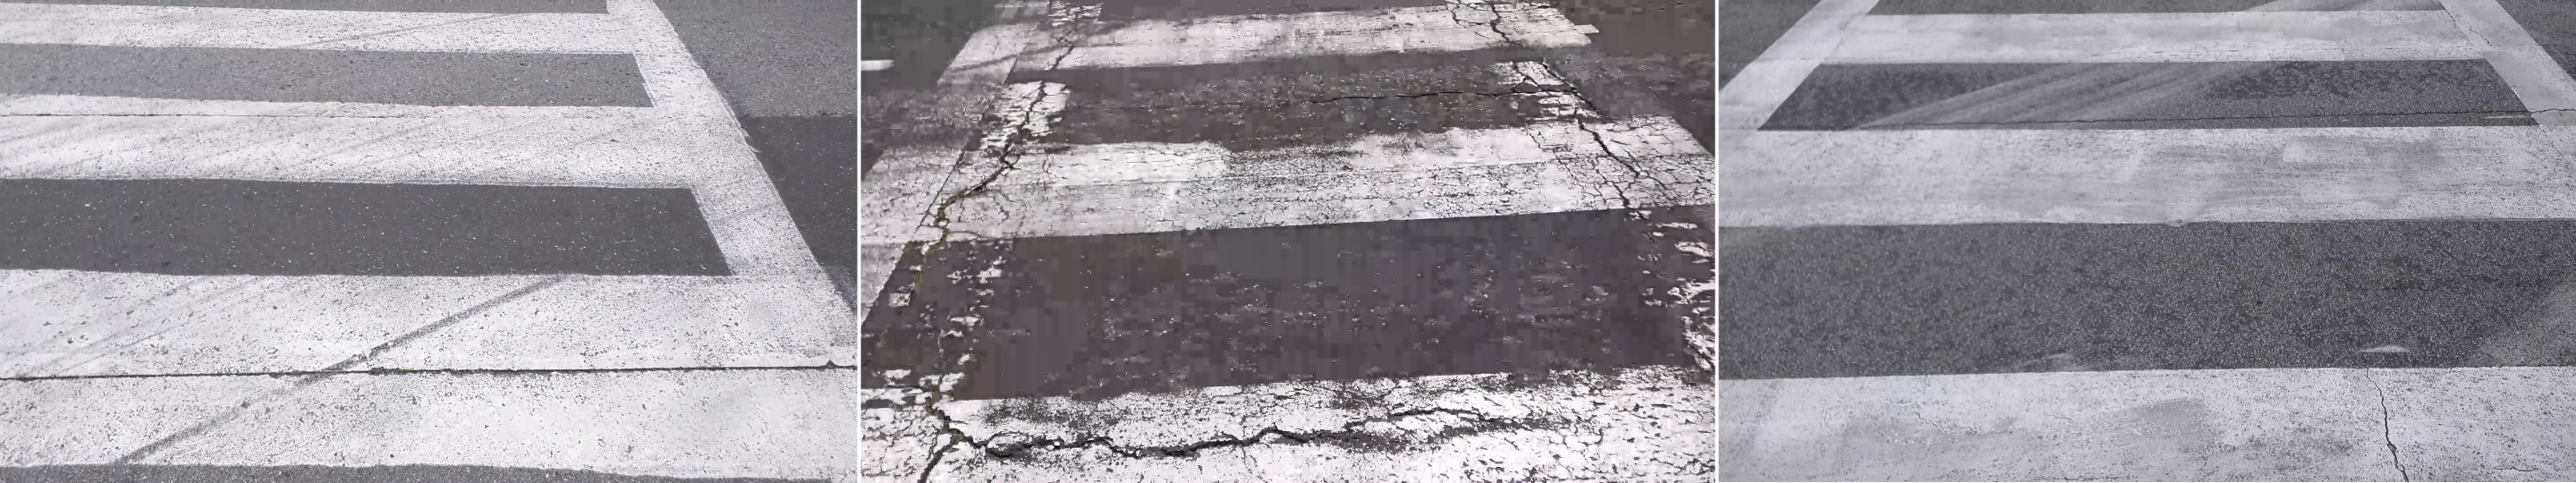
\includegraphics[width=15cm]{figures/DownBad.png}
\captionfonts
\caption{Examples of the low angle video that garnered poor results}
\label{fig:downBadPic}
\end{center}
\end{figure}

\begin{figure}[t]
\begin{center}
\includegraphics[width=15cm]{figures/AllFiveAngles.png}
\captionfonts
\caption{All five angles which videos were taken of the crosswalks. Left to right: (a) Low Angle (b) Left Side (c) Standard (d) Right Side (e) High Angle}
\label{fig:AllFiveAngles}
\end{center}
\end{figure}

\begin{table}[t]
    \begin{longtable}{|r|r|r|}
    \caption{Results of crosswalk detection categorized by video angle}
    \label{tab:downbad}\\

    \hline
    Camera Angle & True Positive Rate & False Positive Rate \bigstrut\\
    \hline
    Low Angle & 45.67\% & 0.00\% \bigstrut\\
    \hline
    Left Side & 77.00\% & 1.00\% \bigstrut\\
    \hline
    Standard & 77.00\% & 0.33\% \bigstrut\\
    \hline
    Right Side & 76.67\% & 1.33\% \bigstrut\\
    \hline
    High Angle & 73.33\% & 0.00\% \bigstrut\\
    \hline
    \end{longtable}
\end{table}

\clearpage

\subsection{Effect of Time of Day}
Each crosswalk was categorized by time of day, morning, midday and night, to see if that had any effect on the prediction rates. The results are shown in table \ref{tab:timeofday}. There were 300 crosswalk frames for each different time of day. The results for each time of day were rather close together, with a slight increase for morning. This might have to do with the lighting causing the image to be more easy to categorize during the morning hours. This data shows that different lighting caused by different time of day did not seem to be a strong factor in the results.

\begin{table}[t]
    \begin{longtable}{|r|r|r|}
    \caption{Results of crosswalk detection categorized by time of day}
    \label{tab:timeofday}\\ 
    \hline
    Time of Day & True Positive Rate & False Positive Rate \bigstrut\\
    \hline
    Morning & 79.09\% & 2.91\% \bigstrut\\
    \hline
    Midday & 75.00\% & 2.05\% \bigstrut\\
    \hline
    Night & 75.44\% & 1.90\% \bigstrut\\
    \hline
    \end{longtable}
\end{table}

\subsection{Zebra Crosswalk Versus Hybrid Crosswalk}

The true positive percent results of zebra stripe and hybrid crosswalks detection are shown in table \ref{tab:typeOfCwalk}. There were nine zebra stripe crosswalks in the dataset, and six hybrids. The least accurately predicted crosswalk was in the hybrid dataset, leading to a much higher standard deviation. The zebra crosswalks were predicted more consistently, leading to a lower standard deviation and higher true positive percents. The training data was biased towards zebra crosswalks, with three hybrids trained versus nine zebra crosswalks. As shown in the table \ref{tab:typeOfCwalk}, the zebra crosswalk median true positive rate only dropped about 3\%, with the introduction of the neural network, while the hybrid median dropped almost 24\% after neural network application. The hybrid crosswalks observed in the area these videos were taken appeared to more frequently have paint irregularities than the zebra crosswalks, as shown in Figure \ref{fig:poorlyPaintedHybrid}, potentially due to different maintenance practices by the municipality, which could also explain the discrepancy. One of the neural network parameters regarding the pixel intensity of the area surrounding the stripelet would also be different for hybrid versus zebra, because hybrids would have a higher value due to the white lines on the sides being part of their surroundings. It is likely that adding more hybrid crosswalks to the training dataset would improve their results.

\begin{figure}[t]
\begin{center}
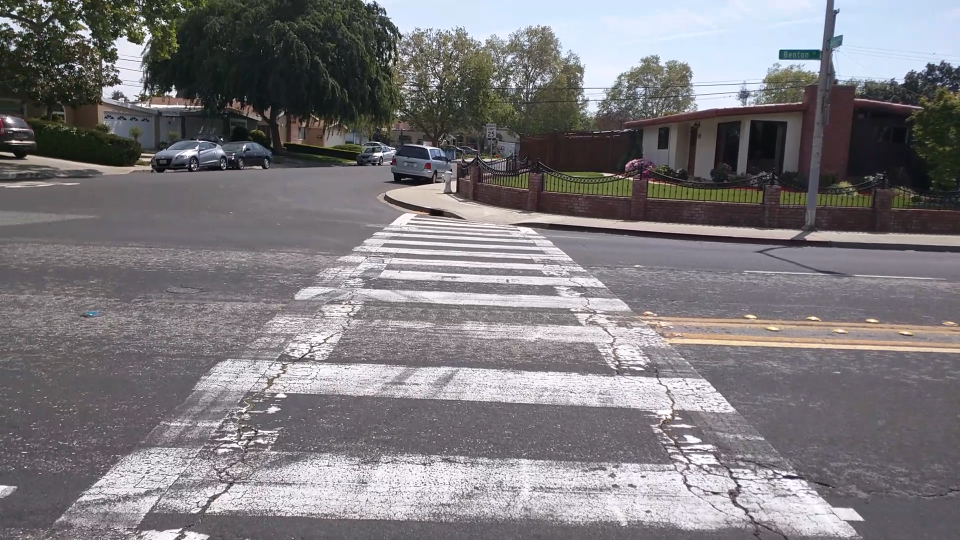
\includegraphics[width=10cm]{figures/PoorlyPaintedHybrid.png}
\captionfonts
\caption{Poorly painted hybrid crosswalk}
\label{fig:poorlyPaintedHybrid}
\end{center}
\end{figure}

\clearpage

\begin{table}[t]
    \begin{longtable}{|r|r|r|r|r|r|r|}
    \caption{True positive percent results of crosswalk detection categorized by type of crosswalk}
    \label{tab:typeOfCwalk}\\ 
    \hline
    Type  & \multicolumn{1}{l|}{Neural Network Enabled} & Min   & Avg   & Median & Max   & STD \bigstrut\\
    \hline
    Hybrid & YES   & 0.00\% & 57.92\% & 62.50\% & 85.00\% & 30.68\% \bigstrut\\
    \hline
    Hybrid & NO    & 15.00\% & 76.46\% & 86.25\% & 98.75\% & 31.18\% \bigstrut\\
    \hline
    Zebra & YES   & 52.50\% & 88.06\% & 95.00\% & 98.75\% & 15.30\% \bigstrut\\
    \hline
    Zebra & NO    & 62.50\% & 92.22\% & 97.50\% & 100.00\% & 11.85\% \bigstrut\\
    \hline
    \end{longtable}
\end{table}

\subsection{Effects of Crosswalk Traversal on Accuracy}

As the user walks across the crosswalk, the view of the crosswalk changes and the algorithm needs to continue guiding them. For each crosswalk, 20 frames equidistant throughout the video were used. The expected result of this is that there would be a decrease in true positive rate as the user progresses because there will be fewer stripelets in the image to work with. The data shown in figure \ref{fig:graphOfFrameCount} shows exactly that. The neural network made the rate go down as one would expect, but the drop seemed to increase as the end of the crosswalk was reached. This may be because the training data may be more biased to earlier frames, since the early frames are guaranteed to have more stripelets. In figure \ref{fig:NumStripeletsvsRates}, we can also see that the number of stripelets in each image as the video went on became fewer as the user crossed the crosswalk, but the predictions of the stripelets stayed mostly consistent throughout. 

\begin{figure}[t]
\begin{center}
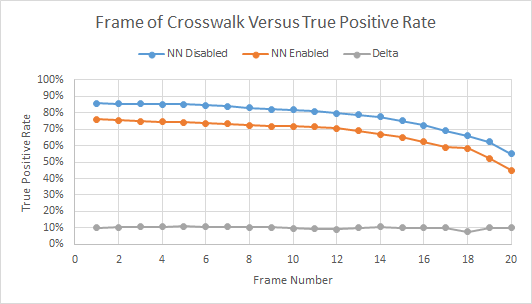
\includegraphics[width=10cm]{figures/FrameResultsGraph.png}
\captionfonts
\caption{True positive results grouped by frame of video (frame 1 to frame 20) as crosswalk is traversed}
\label{fig:graphOfFrameCount}
\end{center}
\end{figure}

\begin{figure}[t]
\begin{center}
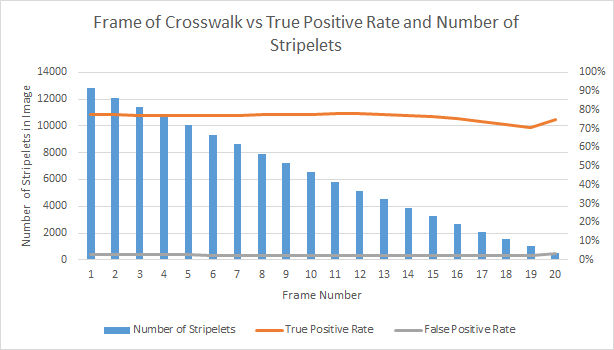
\includegraphics[width=12cm]{figures/NumStripeletsvsRates.png}
\captionfonts
\caption{True and false positive results grouped by frame of video and showing number of detected stripelets (frame 1 to frame 20)}
\label{fig:NumStripeletsvsRates}
\end{center}
\end{figure}

\clearpage

\subsection{Per Crosswalk Analysis of Results}

For this section, the crosswalk videos were grouped by their respective crosswalks, and the non-crosswalk videos were kept as separate groups. The results of this are shown in the appendix tables \ref{tab:appendixcrosswalkresults} and \ref{tab:appendixcrosswalkresultswithoutNeural}, and the summary results are shown in table \ref{tab:crosswalkResultsSummary}. Crosswalks have both true and false positive rates depending on whether they were predicted as being a crosswalk by correct reasoning or not. Videos not containing a crosswalk only have false positives because they cannot contain a crosswalk.  There were a couple outliers in each category (crosswalk vs not) that are included in the dataset, and will be investigated in a later section.

Overall, the average true positive rate of the crosswalk videos was 76\% $\pm$ 13.42\% with a standard deviation of 26.52\%. The average false positive rate of crosswalk images was 0.59\% $\pm$ .64\% with a standard deviation of 1.26\%. The average false positive rate of the non-crosswalk videos was 1.67\% $\pm$ 1.75\% with a standard deviation of 3.45\%.
The true positive predictions of crosswalks had a rather high standard deviation, which was heavily affected by the one outlier crosswalk, and the false positives were more tightly grouped with a lower standard deviation.

\begin{table}[t]
    \begin{longtable}{|r|r|r|r|r|r|r|}
    \caption[Results summary by video/crosswalk]{Results summary by video/crosswalk. Crosswalks have true and false positives, while non-crosswalk videos only have false positives}
    \label{tab:crosswalkResultsSummary}\\
    \hline
          & Cwalk & Minimum & Average & Median & Maximum & STD \bigstrut\\
    \hline
    True Pos Rates & YES   & 0.00\% & 76.00\% & 82.50\% & 98.75\% & 26.52\% \bigstrut\\
    \hline
    False Pos Rates & YES   & 0.00\% & 0.59\% & 0.00\% & 3.75\% & 1.26\% \bigstrut\\
    \hline
    False Pos Rates & NO    & 0.00\% & 1.67\% & 0.00\% & 12.00\% & 3.45\% \bigstrut\\
    \hline
    \end{longtable}
\end{table}



\subsection{Yellow Crosswalks}

In order to determine how well yellow crosswalks worked with white crosswalk training data, two yellow crosswalks were tested, one being a standard zebra and the other a hybrid. The hybrid scored 24\% true positive rate, and the zebra scored 66\%, both out of 80 frames. Those results are promising enough to conclude that yellow crosswalks will likely work well with this approach, and would probably improve with yellow crosswalks being included in the training data, due to the differing intensity values between the two colors affecting neural network parameters. 

\subsection{Challenging Images and Analysis}

The video with the highest amount of false positives (12\%) was `NonC Output Night 13,' which was a street being crossed not at an intersection, and with bike lanes going across both sides. The bike lanes and sidewalk were incorrectly matched together, which ended up passing the neural network and the validation as a crosswalk. A couple examples are shown in figure \ref{fig:worstFalsePosPic}, one can see the identified stripelets. More neural network parameters may be able to help remove these from the stripelet set, perhaps something relating to the vertical pixel intensity. 

\begin{figure}[t]
\begin{center}
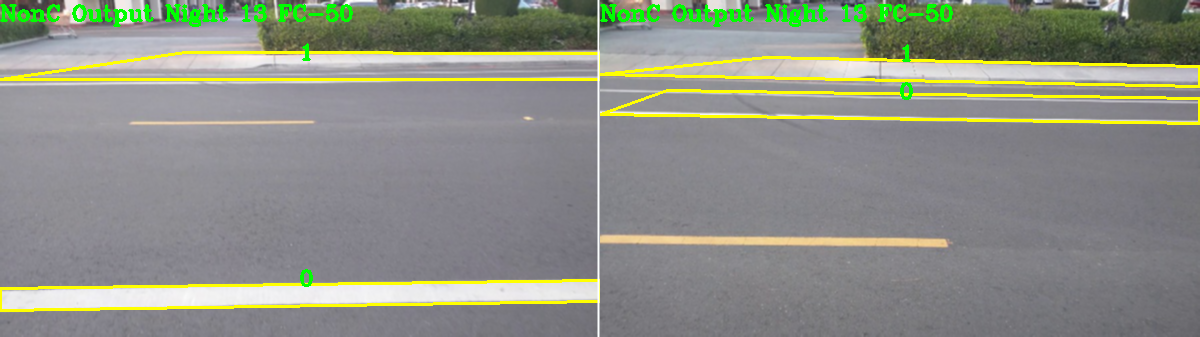
\includegraphics[width=10cm]{figures/NonCWorstCwalk.png}
\captionfonts
\caption{Example frames from 'NonC Output Night 13,' the video with the highest amount of false positives}
\label{fig:worstFalsePosPic}
\end{center}
\end{figure}

Another video with a high amount of false positives (6.67\%) was `NonC Output Night 11,' which is a of a parking lot with many horizontal lines painted throughout.  A few pictures are shown in figure \ref{fig:2ndworstFalsePosPic}. These examples aren't typically what one would expect to see if they were trying to cross the street, but they are lines that look similar to a zebra crosswalk. They could potentially be filtered out by using some sort of expected width vs Y axis level in the image. 

\begin{figure}[t]
\begin{center}
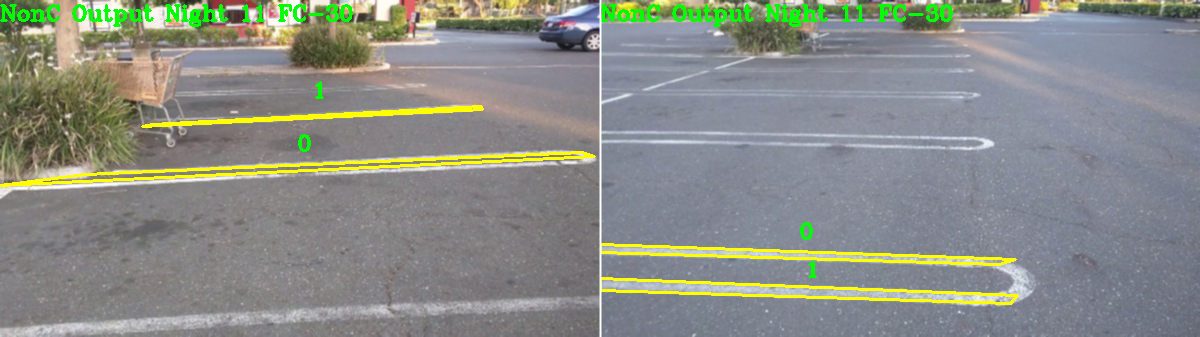
\includegraphics[width=14cm]{figures/NonC2ndWorstCwalk.png}
\captionfonts
\caption{Example frames from 'NonC Output Night 11,' the video with the second highest amount of false positives}
\label{fig:2ndworstFalsePosPic}
\end{center}
\end{figure}

One crosswalk specifically had the worst results by far, 'Night hybrid 3,' shown in figure \ref{fig:worstcwalk}. None of the eighty frames were correctly identified in this crosswalk, whereas the next lowest crosswalk had 53\% of frames correctly identified. The neural network failed to correctly identify enough stripelets in the majority of the images to pass the crosswalk validation. This crosswalk had very odd pavement coloring, which may have contributed to why it failed the neural network.  Potentially this issue could be solved by adding more training data and including more odd crosswalks such as this one. 

\begin{figure}[t]
\begin{center}
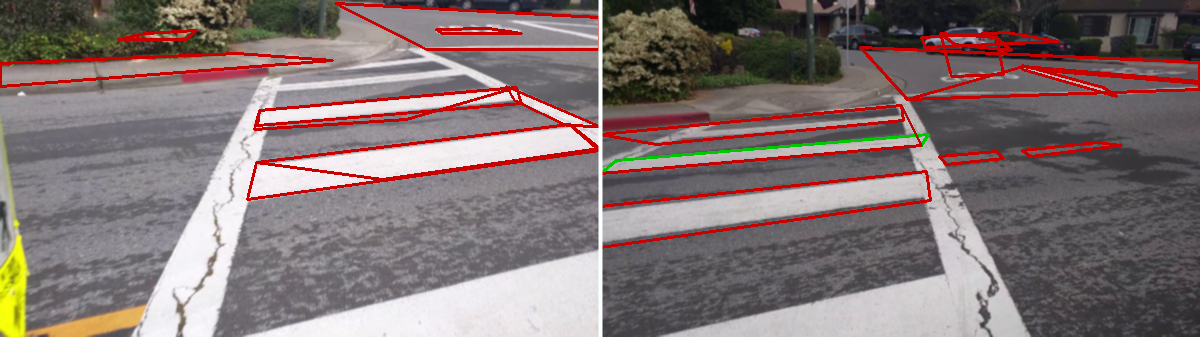
\includegraphics[width=14cm]{figures/WorstCwalk.png}
\captionfonts
\caption{Example frames from 'Night hybrid 3,' the crosswalk with the worst true positive rate}
\label{fig:worstcwalk}
\end{center}
\end{figure}

\clearpage

\subsection{Overall Results}
%\todo[inline]{JASON - Add another evaluation metric here}  
Over all of the videos, including 1200 crosswalk frames and 970 non-crosswalk frames, and using the neural network to cull stripelets before detection, a q-value of .021 is obtained for crosswalk predictions. When not using the neural network to cull the stripelets, the q-value is .200 (see table \ref{tab:overallresults}). Using the neural network garners an improvement of 933\% of this value. In simpler terms, using neural networks, out of 1000 positively predicted images, only 21 would be false positives versus 200 without using the neural predictions. Figure \ref{fig:CrosswalkTruePosWithAndWithout} shows that for every video, the neural network does drop the positive identifications, but figure \ref{fig:VideoFalsePosWithAndWithout} shows that false positive rates dropped drastically as well for every single case. 


\begin{table}[t]
    \begin{longtable}{|r|r|r|r|}
    \caption{Results of crosswalk detection with/without neural networks. Improvement of 937\% in q-value}
    \label{tab:overallresults}\\
    \hline
    \multicolumn{1}{|c|}{Neural Network Enabled} & True Positive Rate & False Positive Rate & q-value \bigstrut\\
    \hline
    NO    & 91.00\% & 24.88\% & 0.200 \bigstrut\\
    \hline
    YES   & 76.51\% & 2.04\% & 0.021 \bigstrut\\
    \hline
    \end{longtable}
\end{table}

\begin{figure}[t]
\begin{center}
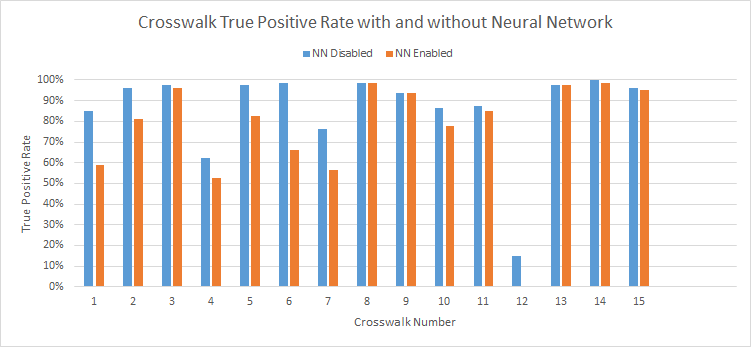
\includegraphics[width=14cm]{figures/CrosswalkTruePosWithAndWithout.png}
\captionfonts
\caption{Shows the true positive rates per crosswalk with and without the neural network enabled}
\label{fig:CrosswalkTruePosWithAndWithout}
\end{center}
\end{figure}

\begin{figure}[t]
\begin{center}
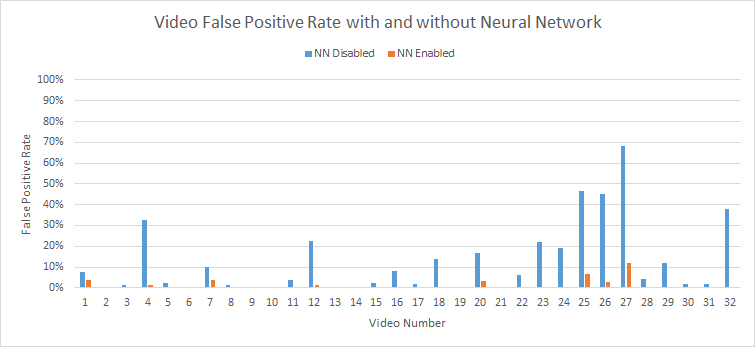
\includegraphics[width=14cm]{figures/VideoFalsePosWithAndWithout.png}
\captionfonts
\caption{Shows the false positive rates per video with and without the neural network enabled}
\label{fig:VideoFalsePosWithAndWithout}
\end{center}
\end{figure}

\subsection{Crosswalk Boundary Line Drawing Results}

A subset of 180 images were selected to test the crosswalk boundary drawing and had their boundary lines manually drawn. A metric was needed in order to compare the correct line with the estimated line. The metric used involved taking multiple points that were equidistant along the estimated line and finding the normal distance to the manually drawn line. These distances were then summed up to give a general gauge of how close lines were together. Exactly identical lines would have a difference value of zero, while more distinct lines would have greater values. Some example images with their evaluation result values are shown in figure \ref{fig:LinesUsingJustGoodStartAndEnds2}. Overall, the results were rather promising, with the vast majority of lines from images with a recognized crosswalk being close to correct with a median measure of 82 and only 16\% of the lines being over the threshold of 400. As shown in figure \ref{fig:400Metric}, 400 was a generous measure, because even at 400, the lines are still close enough.  If the stripelets are predicted properly, and a crosswalk is recognized, the edges of the stripelets are almost guaranteed to be good metrics of the crosswalk edges.

\begin{figure}[t]
\begin{center}
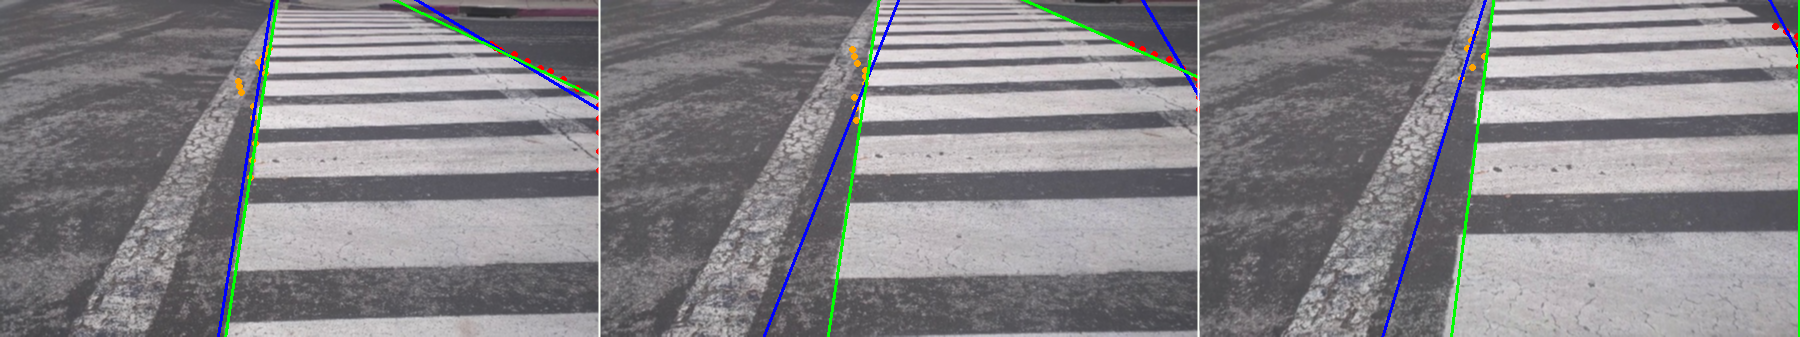
\includegraphics[width=15cm]{figures/LinesUsingJustGoodStartAndEnds2.png}
\captionfonts
%Jeneeplz what term for "left evaluation value"
\caption{Orange and red dots are the right and left points used. Green is the manually drawn boundary. Blue is the estimated boundary. Left to right: (a) Left evaluation metric of 38, right 34. (b) left: 178, right: 135. (c) left: 235, right: 90}
\label{fig:LinesUsingJustGoodStartAndEnds2}
\end{center}
\end{figure}

\begin{figure}[t]
\begin{center}
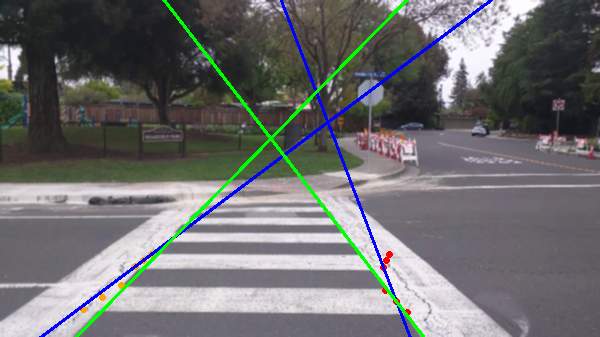
\includegraphics[width=12cm]{figures/400RightSide.png}
\captionfonts
%Jeneeplz what term for "left evaluation value"
\caption{Orange and red dots are the right and left points used. Green is the manually drawn boundary. Blue is the estimated boundary. The evaluation metric on the right side is 400, which is considered the high range of acceptable}
\label{fig:400Metric}
\end{center}
\end{figure}